\documentclass[11pt,t]{beamer}
\mode<presentation> {\usetheme{kuleuven}}
\usepackage[dutch]{babel}
\title{Software-ontwerp}
\author{Castel D., Devlieghere J., Pante S.}
\institute{Groep 25, Computerwetenschappen, KU Leuven}
\subtitle{Finale Presentatie}
\date{24 mei 2013, Leuven, Belgi\"{e}}
\begin{document}
%title page
	\setbeamertemplate{headline}[title_page]
	\setbeamertemplate{footline}[title_page]
	\csname beamer@calculateheadfoot\endcsname %recalculate head and foot dimension
		\begin{frame}
			\titlepage
		\end{frame}
%head and foot for body text	
	\setbeamertemplate{headline}[body]
	\setbeamertemplate{footline}[body]

\section{Werkverdeling}

\begin{frame}{Werkverdeling}
\end{frame}

\section{Testen}

\begin{frame}{Testen}
\end{frame}

\section{Domain Model}



\begin{frame}{Domain Model}

\begin{center}
\begin{figure}
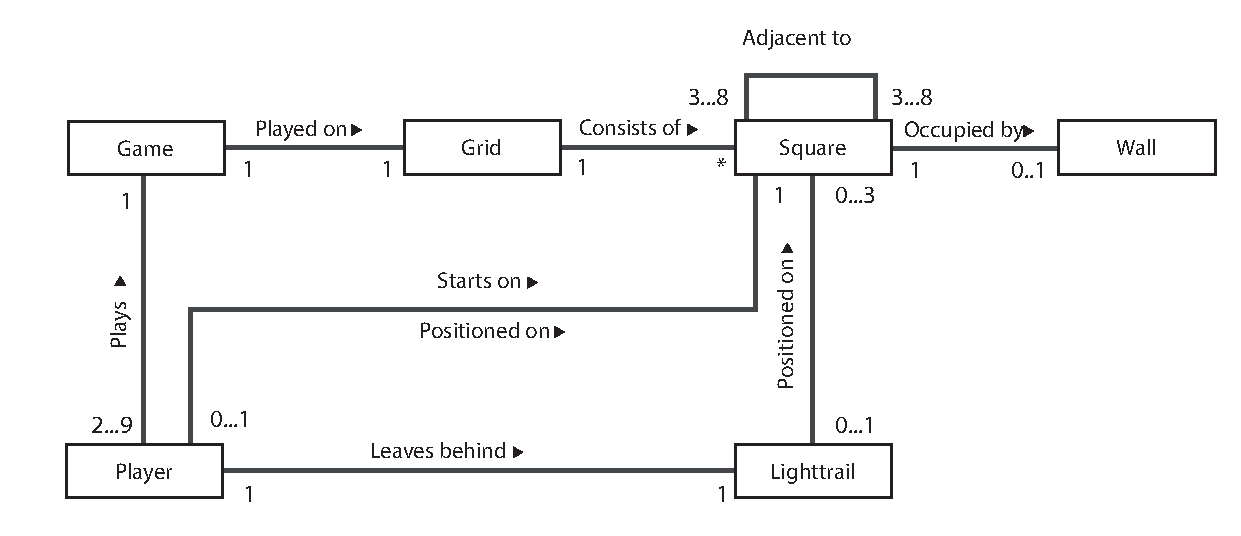
\includegraphics[width=0.9\linewidth]{images/domainmodel2}
\end{figure}
\end{center}
\begin{itemize}
\item 2..9 players
\item 1..8 adjacent squares, mogelijk bij grids gebouwd van file
\end{itemize}
\end{frame}

\begin{frame}{Domain Model}
\begin{center}
\begin{figure}
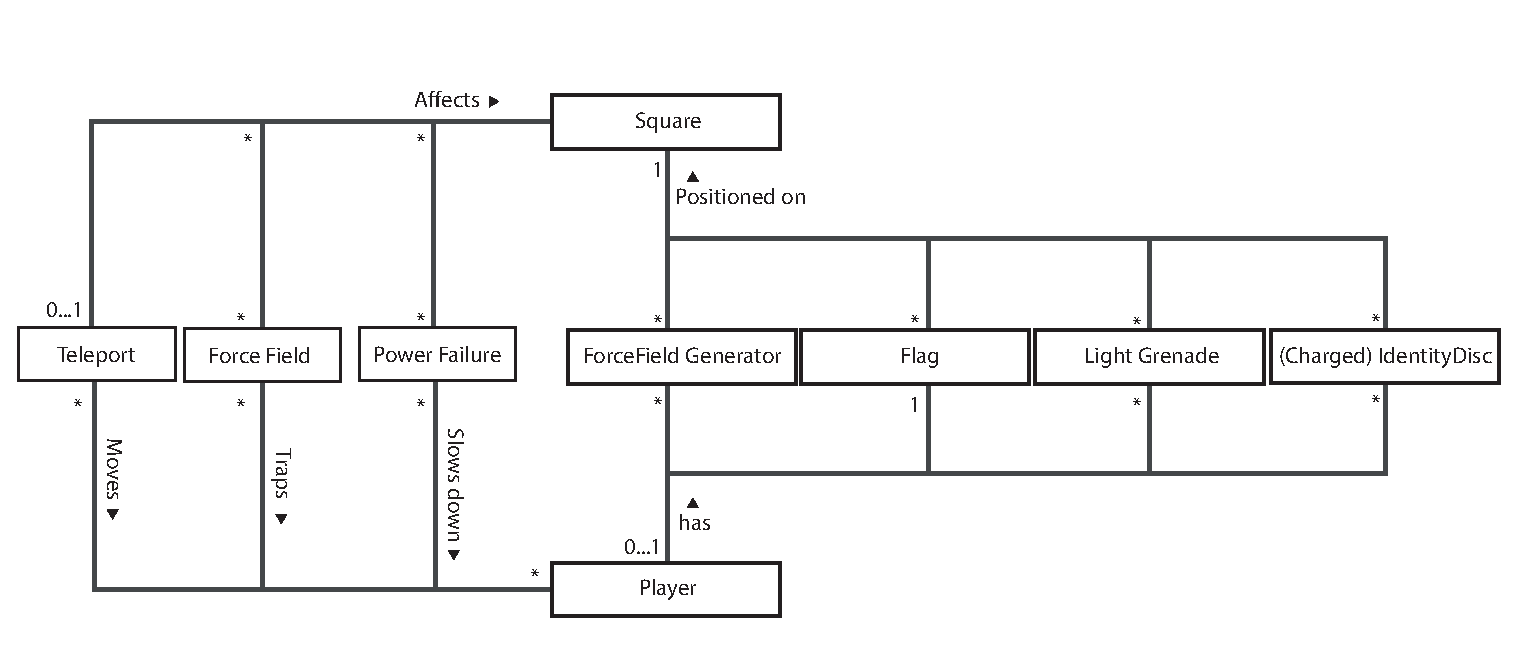
\includegraphics[width=0.9\linewidth]{images/domainmodel1}
\end{figure}
\end{center}
\begin{itemize}
\item Toevoeging van concept voor Flag, Teleport, Forcefield, IdentityDisc.
\item Player kan maximum 1 vlag dragen!
\end{itemize}


\end{frame}

\begin{frame}{Domain Model}
\begin{center}
\vspace{0.9in}
\begin{figure}
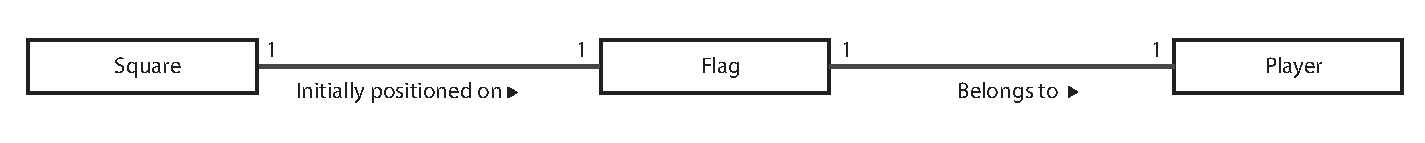
\includegraphics[width=1\linewidth]{images/domainmodel3}
\end{figure}
\end{center}
\begin{itemize}
\item Een Flag is initieel op een square geplaatst 
\item Flag is eigendom van \'{e}\'{e}n speler
\end{itemize}
\end{frame}

\section{Implementatie}

\subsection{Grid}

\begin{frame}{GridElements}
\end{frame}

\begin{frame}{Coordinate}
\end{frame}

\begin{frame}{Square}
\end{frame}

\begin{frame}{Wall}
\end{frame}

\begin{frame}{GridBuilder}
\begin{center}
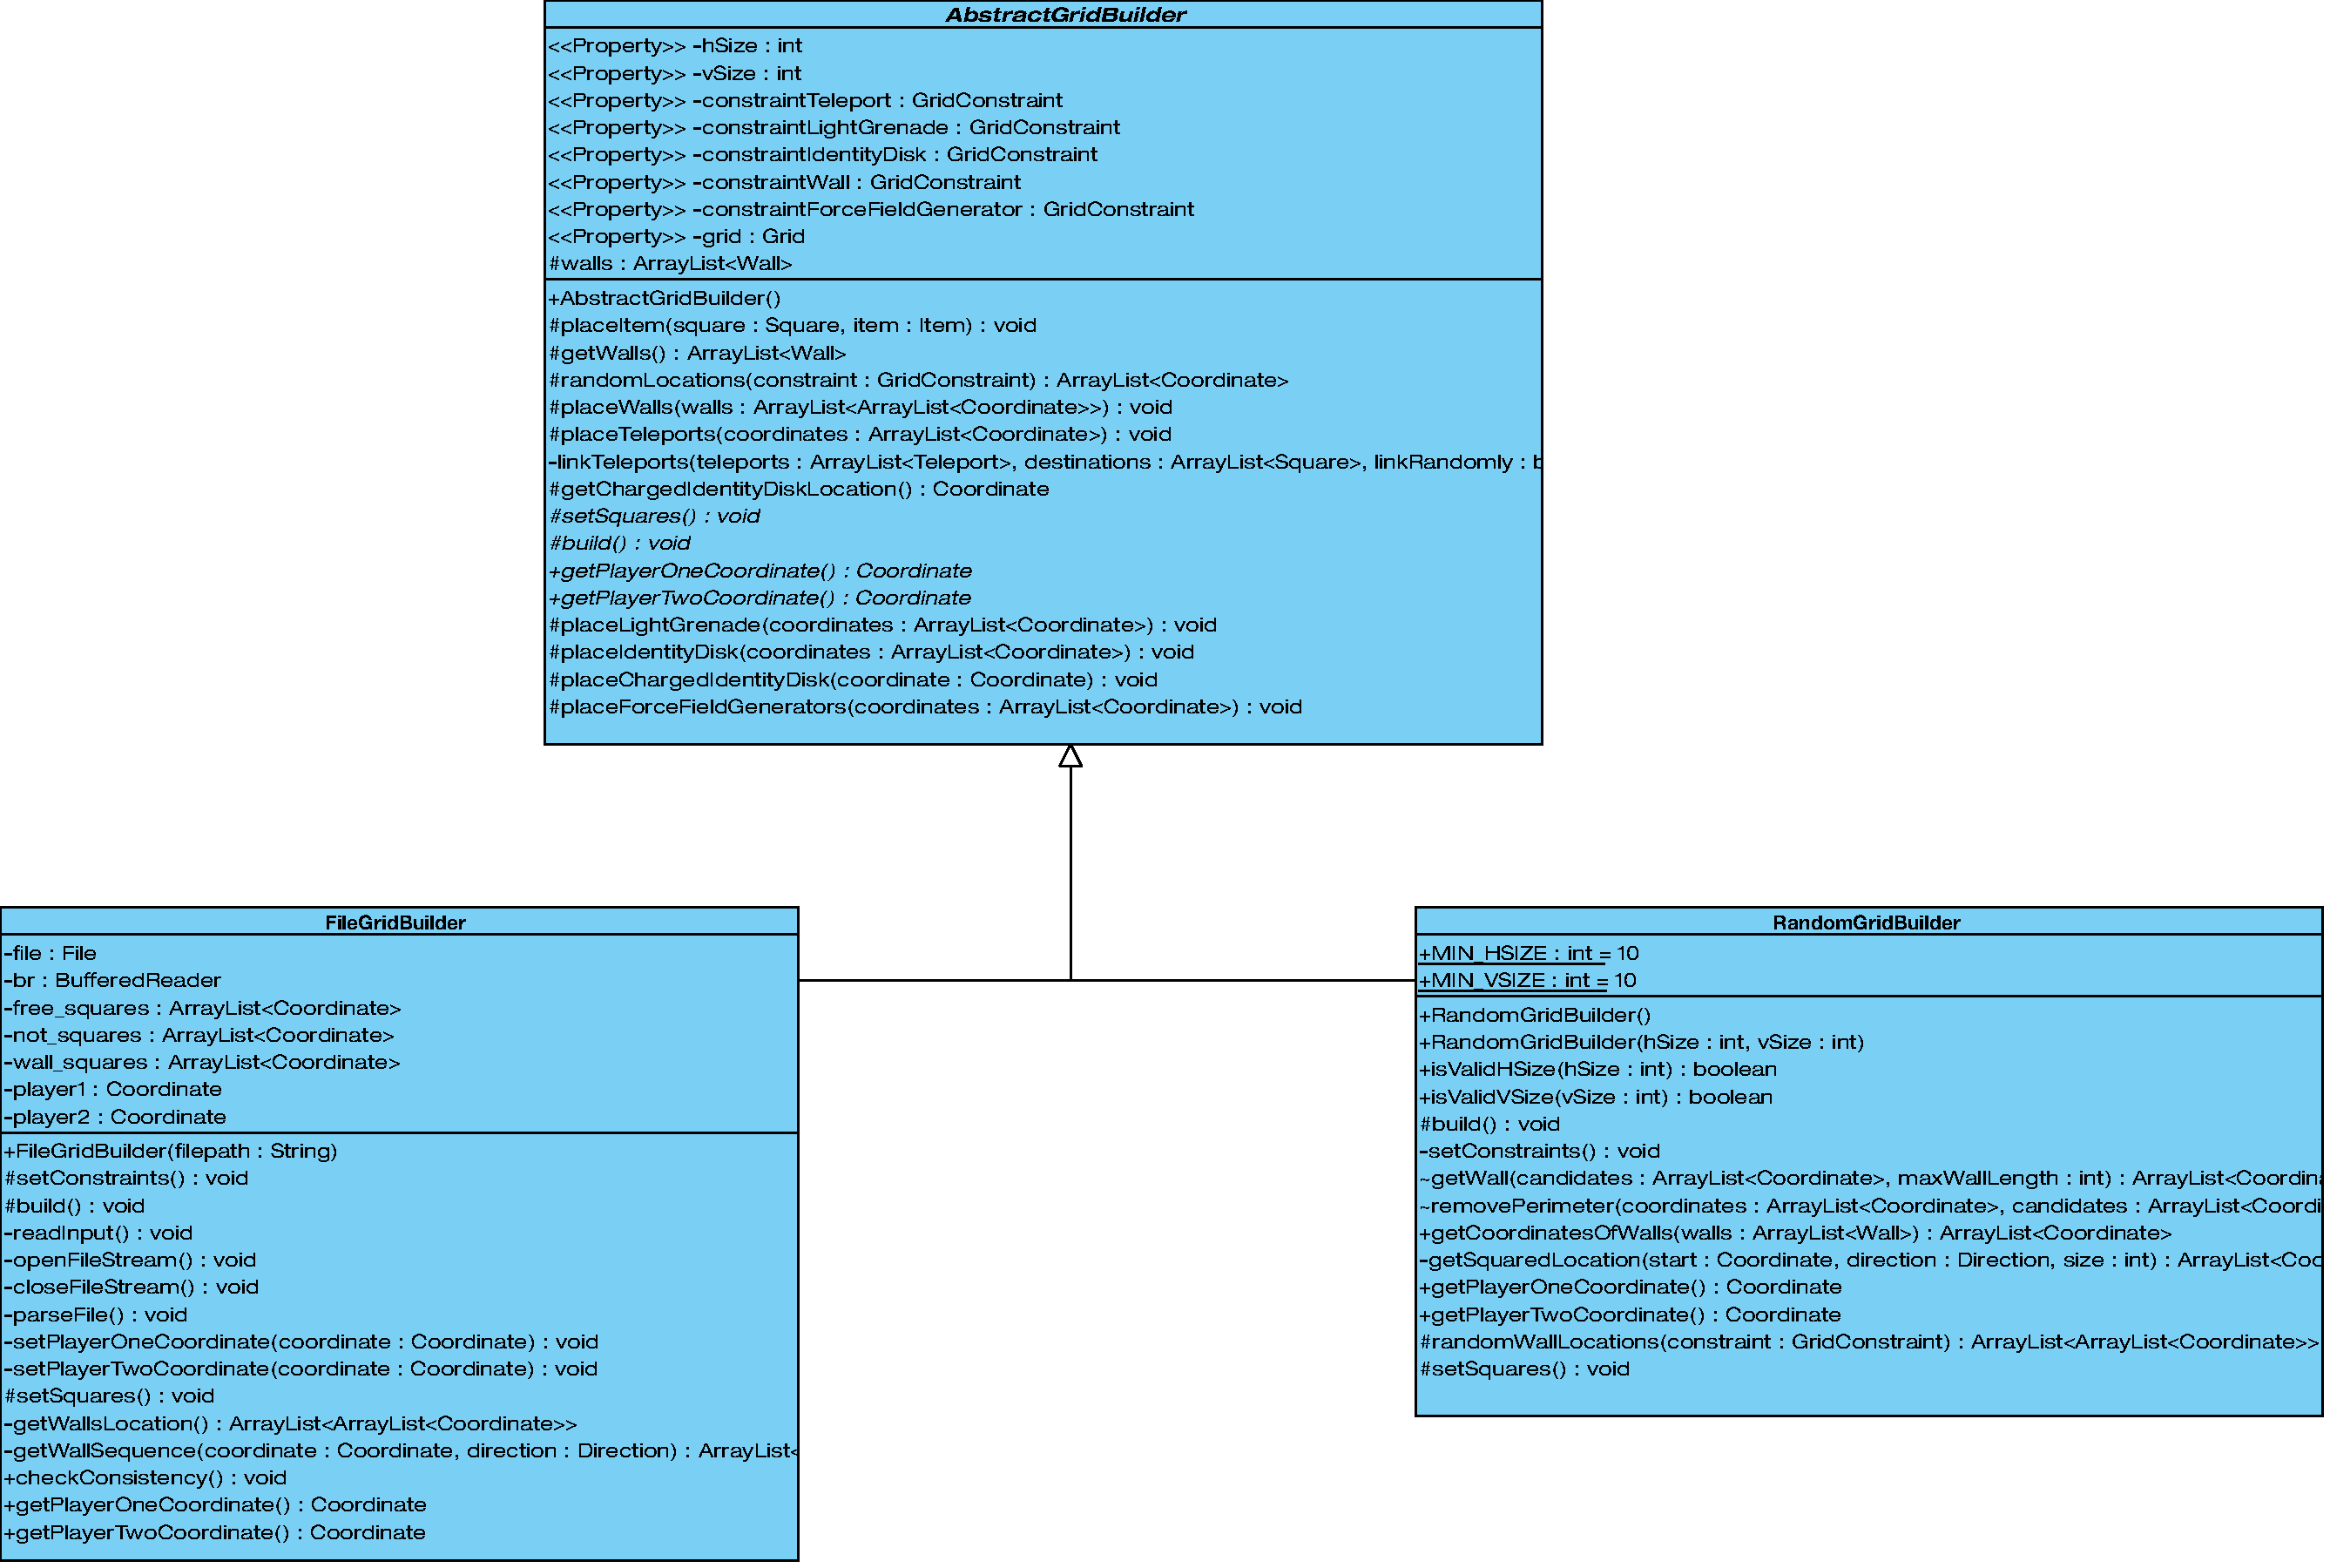
\includegraphics[width=1\linewidth]{images/gridbuilder}
\end{center}
\end{frame}

\subsection{Items}

\begin{frame}{Items}
\end{frame}

\begin{frame}{LightGrenade}
\end{frame}

\begin{frame}{IdentityDisc en ChargedIdentityDisc}
\end{frame}

\begin{frame}{ForceFieldGenerator}
\end{frame}

\begin{frame}{Flag}
\end{frame}

\begin{frame}{Itemplacer}
\end{frame}

\subsection{Effecten}

\begin{frame}{LightTrail}
\end{frame}

\begin{frame}{PowerFail}
\end{frame}

\begin{frame}{Teleport}
\end{frame}

\subsection{Game}

\begin{frame}{Player}
\end{frame}

\begin{frame}{Game}
\end{frame}

\begin{frame}{RaceGameMode}
\end{frame}

\begin{frame}{CTFGameMode}
\end{frame}

\subsection{Acties}

\begin{frame}{Command (Command pattern)}
\end{frame}

\begin{frame}{Move}
\end{frame}

\begin{frame}{Pick Up}
\end{frame}

\begin{frame}{Use Item}
\end{frame}

\begin{frame}{Throw IdentityDisc}
\end{frame}

\begin{frame}{End Turn}
\end{frame}

\subsection{Handlers}

\begin{frame}{Handlers}
\end{frame}

\begin{frame}{Overview (Model view adapter pattern)}

\end{frame}
\section{Slot}
\begin{frame}
\vspace{1.5in}
\begin{center}
Bedankt voor uw aandacht.
\end{center}
\end{frame}
\end{document}